\documentclass[a4paper,UTF8]{article}
\usepackage{ctex}
\usepackage[margin=1.25in]{geometry}
\usepackage{color}
\usepackage{graphicx}
\usepackage{amssymb}
\usepackage{amsmath}
\usepackage{amsthm}
%\usepackage[thmmarks, amsmath, thref]{ntheorem}
\theoremstyle{definition}
\newtheorem*{solution}{Solution}
\newtheorem*{prove}{Proof}
\usepackage{multirow}
\usepackage{url}
\usepackage{enumerate}
\usepackage{listings}
\usepackage{caption}
\usepackage{subfigure}
\usepackage[colorlinks,linkcolor=black, anchorcolor=black,citecolor=black,]{hyperref}


\begin{document}
\title{\textbf{《计算机图形学》十月报告}}
\author{学号:181860077 姓名:佘帅杰,\href{mailto:3121416933@qq.com}{3121416933@qq.com}}
\maketitle

\section{综述}
注:本次报告是增量式的报告,即本次的报告内内容就是这个月做的内容,不包含上个月已经报告过的任何内容

\begin{enumerate}
    \item 实现Bezier曲线绘制算法
    
    \item 实现B-Spline曲线绘制算法
    
    \item 在CLI做对应的处理,加入曲线绘制算法的对应功能

    \item 实现对图元的平移,旋转,缩放以及裁剪的操作,至此已经实现了所有算法模块里的内容
    
    \item 对CLI中添加对图元操作的相关支持
\end{enumerate}


\section{算法介绍}
\subsection{曲线的参数化表示}
在绘制曲线之前,首先需要了解怎么对曲线进行参数化的表示
实际上对于表示一条曲线的各个变量,都可以用某个参数的函数来表示
$$
\begin{cases}
    x=x(u)\\
    y=y(u)\\
    z=z(u)
\end{cases}
$$

三个坐标分量就组成曲线上该点的位置矢量,曲线就可表示为参数u的矢函数
通过这个对曲线进行参数化表示,也是后面绘制曲线的算法的重要基础
对应的图元的生成就可以看作是这个联结的变量的变化过程

\subsection{Bezier曲线绘制算法}
一阶的Bezier曲线就是一条直线,相当于是在两个控制点之间做插值,最后相当于是一个点在两个点之间移动。
最后他的轨迹就是一条直线,也就是两个控制点之间的曲线。这个过程使用公式可以表达为:$ B_{1}(t)=P_0+(P_1-P_0) t$。这里的t可以和上文的
曲线参数化表示关联,t就是那个负责联结的参数。
对于有三个控制点的情况,这个时候是二阶的Bezier曲线,可以看作是两层的一阶Bezier曲线,基本的理解方式可以看到下面的图

\begin{figure}[h]
	\centering
	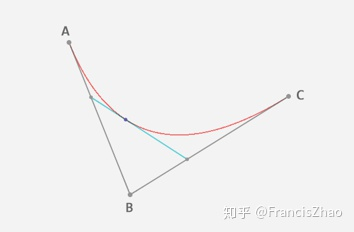
\includegraphics[scale=0.8]{figure/b.png}
	\caption{二阶Bezier算法理解图}
	\label{fig:bezier-alg}
\end{figure}

上述的图可以看出整个过程还是一个插值的过程,在一次插值的结果的基础上做了第二次插值得到结果
同理的更加高阶的Bezier都能够一步一步的降阶
整个过程还可以发现到系数是二项式的展开,进而得到公式实现算法。\\

$$f(x)=
\begin{cases}
    P_{i}  \\
    (1-u)P_{i}^{r-1}+(1-u)P_{i+1}^{r-1}
\end{cases}
$$
对应的图片
\begin{figure}[h]
	\centering
	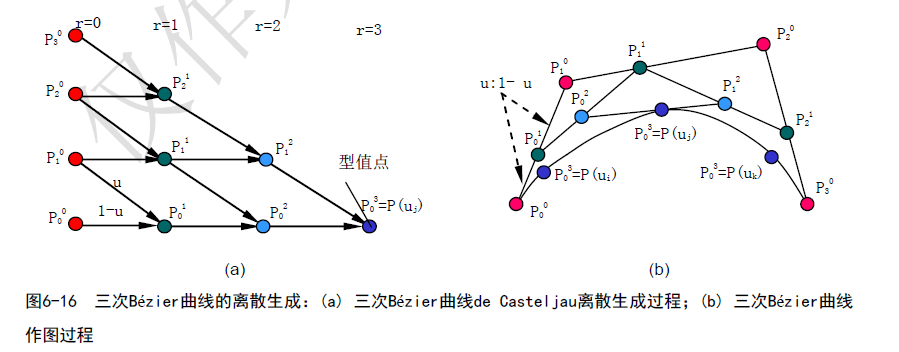
\includegraphics[scale=0.6]{figure/bezier2.png}
	\caption{Bezier算法演示图}
	\label{fig:bezier2}
\end{figure}

算法使用过的指令文件:\\

resetCanvas 600 600\\

setColor 0 255 0\\

drawCurve curve1 50 200 100 100 150 200 Bezier\\

drawCurve curve2 50 400 100 300 150 400 200 300 Bezier\\

saveCanvas 5\\

算法结果:\\
\begin{figure}[h]
	\centering
	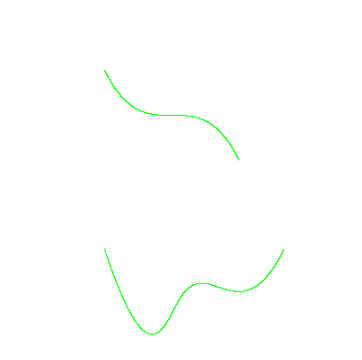
\includegraphics[scale=0.8]{figure/bezier.png}
	\caption{Bezier算法测试结果图}
	\label{fig:bezier-result}
\end{figure}

\subsection{B-spline曲线绘制算法}
\par B样条曲线算法涉及到了基函数:什么是基函数?
基函数 就是一个函数的固定形式,也就是函数只会在这个函数的基础上变化而不会丢掉的函数,在数学中,
基函数是函数空间一组特殊的基的元素。对于函数空间中的连续函数都可以表示成一系列基函数的线性组合,
就像是在向量空间中每个向量都可以表示成基向量的线性组合一样。
\par 同时由于Bezier算法本身的一些问题如:缺少局部性,不够灵活等等,所以B样条出现
虽然上面说了B样条有所不同,但是B样条的本质还是一个降阶然后解决问题的过程。
$$
P(t)=
\begin{bmatrix} 
    t^3 & t^2 & t & 1 
\end{bmatrix}
\begin{bmatrix} 
    -1 & 3 & -3 & 1 \\ 
    3 & -6 & 3 & 0 \\ 
    -3 & 0 & 3 & 1 \\ 
    1 & 4 & 1 & 0 \\ 
\end{bmatrix}
\begin{bmatrix} 
    p_0 \\ 
    p_1 \\ 
    p_2 \\ 
    p_3 \\ 
\end{bmatrix}
$$
基于上述的公式可以在四个控制点的三次B样条进行绘制曲线,但是在实际的情况里
控制点可能不止4个,对应的方法就是利用一个移动的窗口在控制点数组上滚动,举个例子就是
1,2,3,4,5,得到对应的窗口1,2,3,4和2,3,4,5。这样得到的曲线每一段
都能够自然衔接,同时具有连续性。下面的图也可以做辅助说明
\begin{figure}[h]
	\centering
	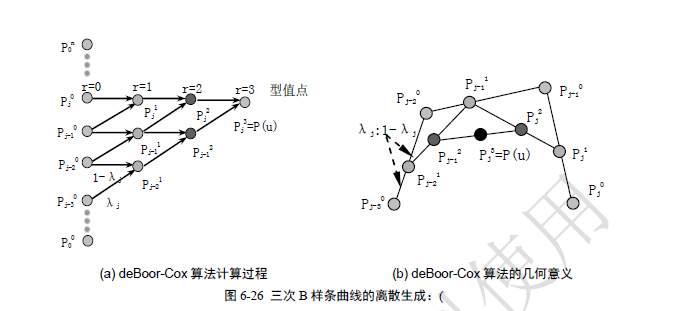
\includegraphics[scale=0.6]{figure/b-spline.png}
	\caption{B-spline算法示意图}
	\label{fig:b-spline-alg}
\end{figure}

实现之后使用算法进行测试,测试语句如下:\\

resetCanvas 600 600\\

setColor 0 0 255\\

drawPolygon polygon2 250 400 300 300 350 400 400 300 Bresenham\\

setColor 0 0 0\\

drawCurve curve3 250 400 300 300 350 400 400 300 B-spline\\

setColor 0 0 255\\

drawPolygon polygon3 250 200 300 50 350 250 400 100 450 200 Bresenham\\

setColor 0 0 0\\

drawCurve curve4 250 200 300 50 350 250 400 100 450 200 B-spline\\

saveCanvas 5\\

测试的结果如下
\begin{figure}[h]
	\centering
	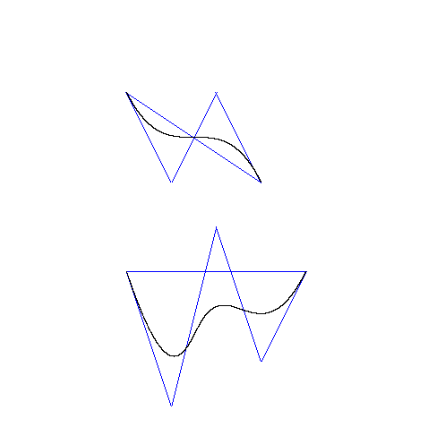
\includegraphics[scale=0.6]{figure/b-spline-result.png}
	\caption{B-spline测试结果图}
	\label{fig:b-spline-result}
\end{figure}

\subsection{图元平移算法}
平移严格的说是把一个点沿着直线路径从一个坐标位置移动到另一个坐标位置的重定位的
过程,说的简单的一些就是,图元的平移就是相对简单一些,图元的构造来源于传入的参数,即“控制点”
相对的,如果想要图元的位置进行平移,只需要对图元的控制点进行操作,
进行对应的平移,则最后的图形也会做对应的平移
算法的测试如下:使用如下的测试指令:\\

resetCanvas 600 600\\

setColor 0 255 0\\

drawLine line1 0 0 500 250 DDA\\

setColor 255 0 0\\

drawLine line2 0 0 500 250 Bresenham\\

translate line2 0 50\\

saveCanvas 1\\

测试的结果如下
\begin{figure}[h]
	\centering
	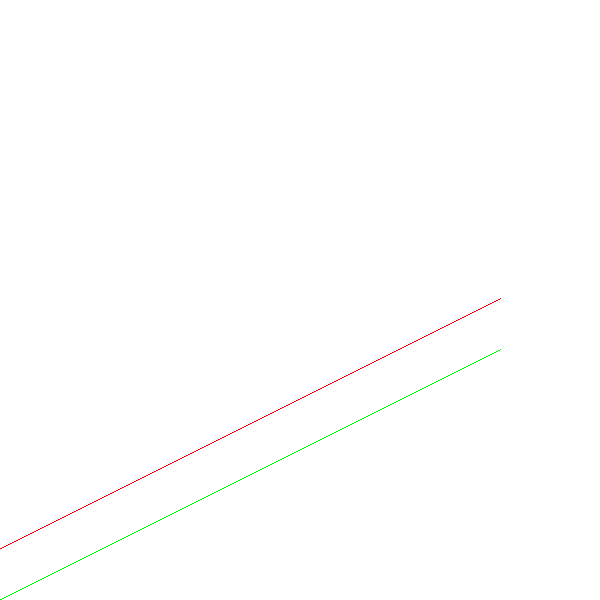
\includegraphics[scale=0.4]{figure/1.png}
	\caption{平移算法测试示意图}
	\label{fig:Rotate}
\end{figure}

\subsection{图元旋转算法}
旋转变化主要是二维的,就是把坐标点关于某个位置转动一个角度,然后确定新的坐标位置的
过程,对应也有公式可以进行参考,对应的公式参考如下:

\begin{figure}[h]
	\centering
	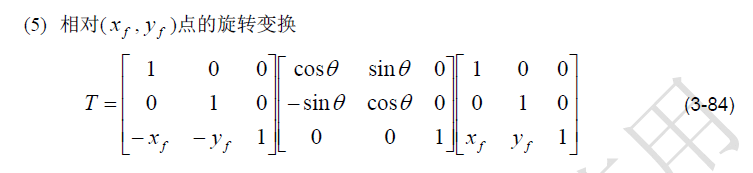
\includegraphics[scale=0.5]{figure/rotate.png}
	\caption{旋转公式图}
	\label{fig:rotate-alg}
\end{figure}

然后对应的对算法进行测试,使用的测试指令文件基本如下\\

resetCanvas 600 600\\

setColor 0 255 0\\

drawLine line1 100 100 400 300 DDA\\

setColor 0 255 255\\

drawLine line2 100 100 400 300 DDA\\

rotate line1 100 100 45\\

saveCanvas 1\\

\begin{figure}[h]
	\centering
	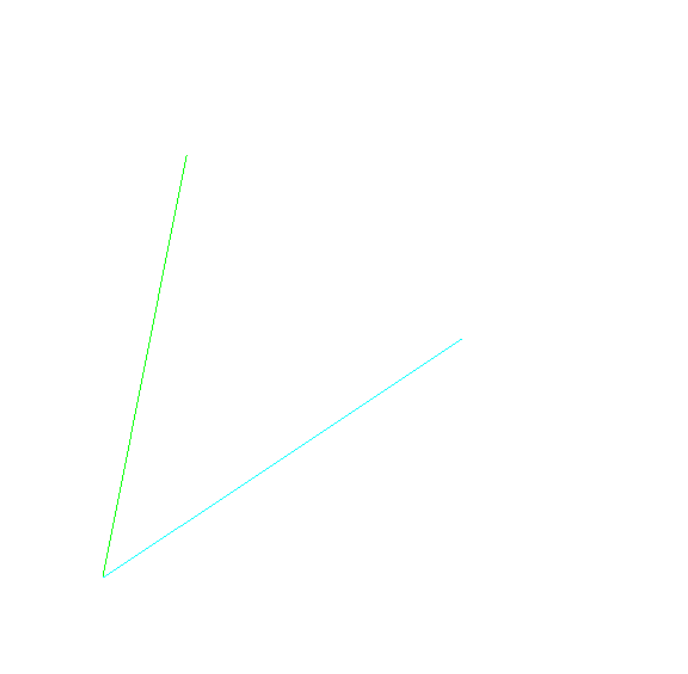
\includegraphics[scale=0.4]{figure/rotate_test.png}
	\caption{旋转算法测试结果图}
	\label{fig:rotate-result}
\end{figure}

\subsection{图元缩放算法}
同上所述,图元的构造主要来自于控制点的限制,对应的可以对控制点的位置进行修改,
缩放可以得到一个缩放的中心和倍数,对每一个控制点,查看其到缩放中心的位置,然后
把这个位置乘上缩放的倍数就可以很直观的看到,整个图形沿着缩放中心缩小或者是放大的
现象,这个算法相对也要简单一些

\begin{figure}[ht]
	\centering
	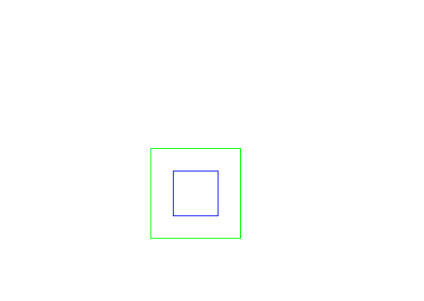
\includegraphics[scale=0.5]{figure/scale.png}
	\caption{缩放测试结果图}
	\label{fig:scale-alg}
\end{figure}

\subsection{图元裁剪算法}
识别图元在指定区域内外部的算法叫做裁剪,用来裁剪对象的区域被称为裁剪窗口。
当给定图元和裁剪窗口之后只留下(显示)给定的范围内的部分,而对于区域外的部分则
不予显示,
图元的裁剪算法很多,但是由于有很多的图元需要执行裁剪操作,对裁剪算法的效率有比较高的
要求
\subsubsection{Cohen-Sutherland算法}
这个算法的的基本思路就是对整个曲线进行了切分和分类,可以比较显示和可理解的
表示出一个线段和裁剪窗口之间的位置关系,对于完全在内部和外部的线段可以快速
判断而提高效率,编码的方式可见下图
\begin{figure}[h]
	\centering
	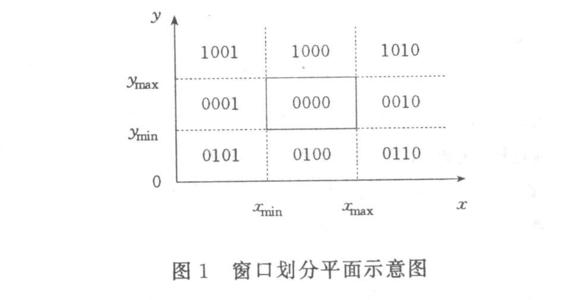
\includegraphics[scale=0.4]{figure/2.png}
	\caption{裁剪区域编码示意图}
	\label{fig:Rotate}
\end{figure}
然后可以直接通过比较或者是作差得到对应的区域码,对得到的两个区域码执行对应的计算
来判断直线和裁剪窗口的对应关系,比如说二者的区域码都是0000则说明整个线段都在裁剪
窗口里。或者是二者相与的结果不是0000,则说明整个线段都在区域外。\\
上述的两种情况是相对简单的两种,都不需要做相对复杂的操作,对于比较复杂度情况
就是有一部分的线在区域内,这就需要求解交点等操作,基本的思路就是求交点,然后确定
那一部分是要被丢弃的,然后在剩余的部分继续做求解\\
使用下述的指令文件进行测试:\\

resetCanvas 600 600\\

setColor 0 255 0\\

drawLine line1 0 0 500 250 DDA\\

setColor 255 0 0\\

drawLine line2 0 0 500 250 Bresenham\\

translate line2 0 50\\

clip line2 50 50 400 200 Cohen-Sutherland\\

drawPolygon polygon4 50 50 400 50 400 200 50 200 Bresenham\\

saveCanvas 1\\

对应的测试结果如下:\\

\begin{figure}[h]
	\centering
	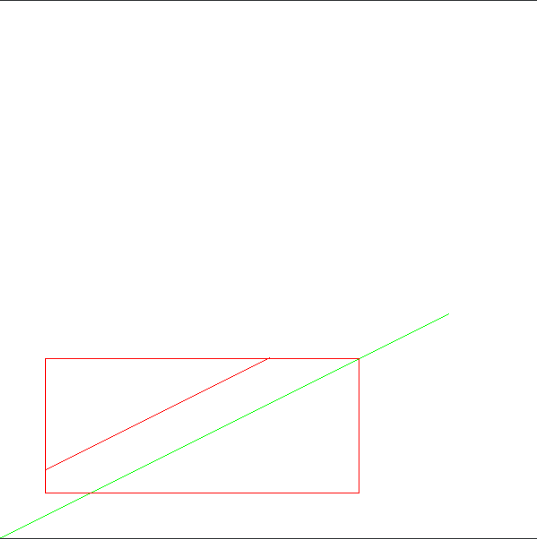
\includegraphics[scale=0.4]{figure/clip1.png}
	\caption{Cohen-Sutherland算法测试结果}
	\label{fig:Cohen-Sutherland算法剪切}
\end{figure}

\subsubsection{梁友栋-Barsky算法}
这个算法的最基本的思路把点和面都看作是大量的
点的集合,然后裁剪的结果就应该是二者的交集

类似的,这个裁剪算法也是用了一些参数来判断二者的相对的关系,基本的示意图如下
\begin{figure}[h]
	\centering
	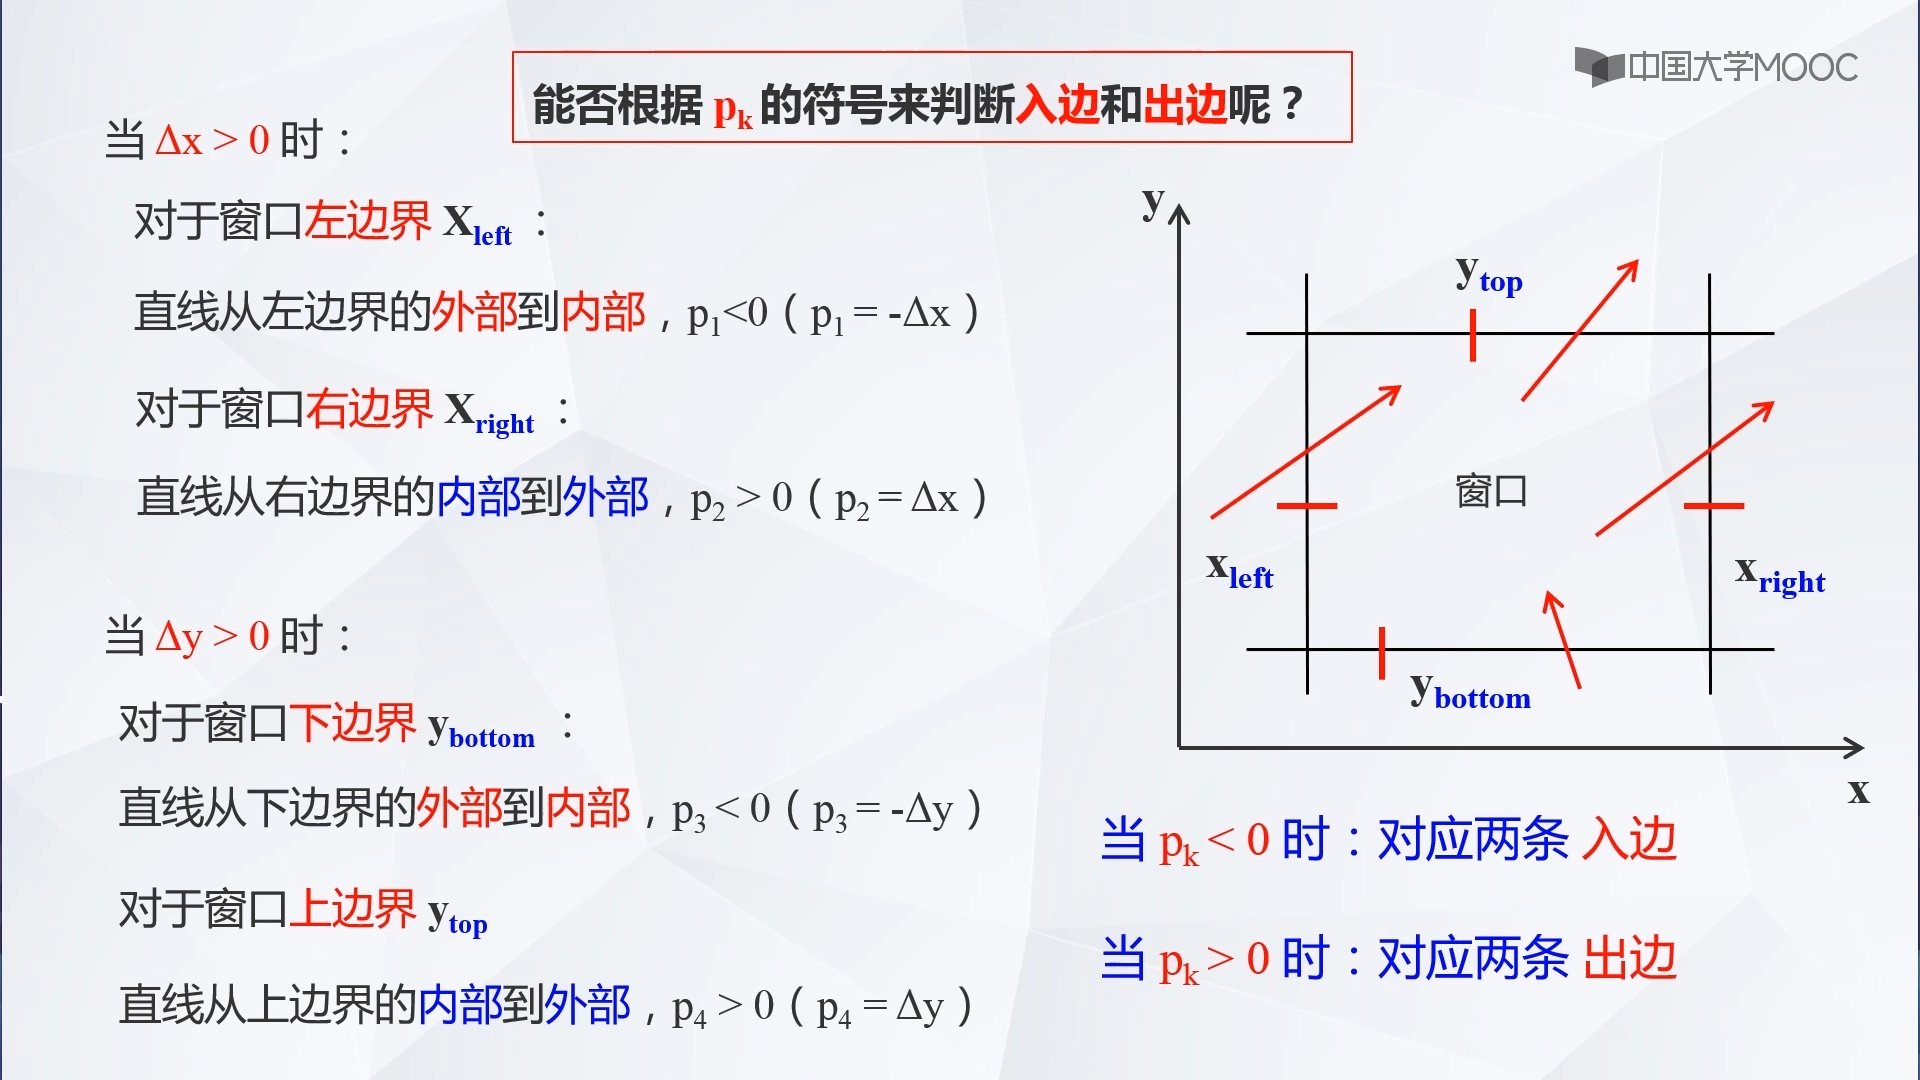
\includegraphics[scale=0.2]{figure/example.png}
	\caption{梁友栋-Barsky算法示意图}
	\label{fig:Barsky}
\end{figure}
对应的使用了好几个变量,包括 $\delta x$表示的是直线左右上的方向
然后对应的$\delta y$ 上下的方向。具体的公式如下\\
$$
\begin{cases}
    p1 = - \Delta x \\
    p2 = \Delta x\\
    p3 = - \Delta y \\
    p4 = \Delta y\\
    q1 = x_{1} - x_{left} \\
    q2 = x_{right} - x_{1}\\
    q3 = y_{1} -y_{bottom} \\
    q4 = y_{top} - y_{1}\\
\end{cases}
$$
对应的对上述的参数的数值进讨论可以得到线段和裁剪窗口的相对的位置关系

\begin{itemize}
    \item [(1)] 
    若pk=0,直线平行于裁剪边界之一。此时,如果同时满足qk<0,则线段完全在
    边界外;如果同时满足qk≥0,线段平行于裁剪边界,并且在窗口内;这种情况是相对简单一些的情况
    \item [(2)]
    当pk<0, 线段从裁剪边界延长线的外部延伸到内部
    \item [(3)]
    当pk>0,线段从裁剪边界延长线的内部延伸到外部
  \end{itemize}

对应的算法伪代码
\begin{itemize}
    \item [(1)] 
    将线段交点的参数初始化为 u1=0,u2=1;
    \item [(2)]
    定义一个函数,用 p、q 来判断是舍弃线段还是改变交点的参数r:
    当p<0 时,参数r 用于更新u1;
    当p>0 时,参数r 用于更新u2:
    如果更新u1 或u2 后使u1>u2,则舍弃该线段;
    否则,更新适当的u 值仅仅求出了交点,缩短线段。
    \item [(3)]
    p、q 的四个值经过测试后,当p=0 且q<0 时,说明该线段平行于边界且位于边
    界之外,舍弃该线段。假如该线段未被舍弃,则裁剪线段的端点由u1、u2 值决定。
    \item [(4)]
    反复调用算法进行计算
  \end{itemize}

使用下述的指令文件进行测试:\\

resetCanvas 600 600\\

setColor 0 255 0\\

drawLine line1 0 0 500 250 DDA\\

setColor 255 0 0\\

drawLine line2 0 0 500 250 Bresenham\\

translate line2 0 50\\

clip line2 50 50 400 200 Liang-Barsky\\

drawPolygon polygon4 50 50 400 50 400 200 50 200 Bresenham\\

saveCanvas 1\\

最后的测试结果

\begin{figure}[h]
	\centering
	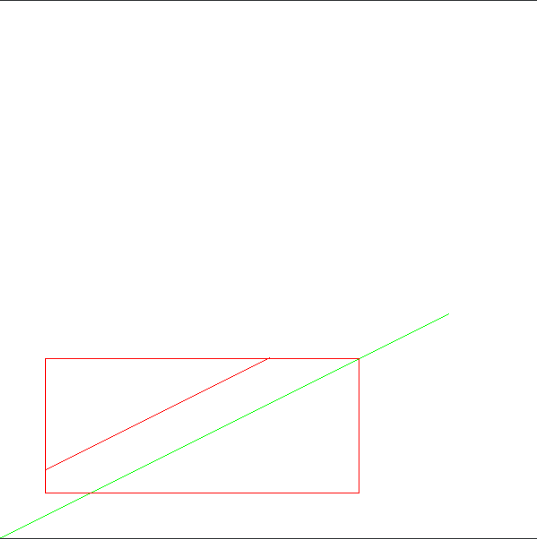
\includegraphics[scale=0.4]{figure/clip1.png}
	\caption{Liang-Barsky算法测试结果}
	\label{fig:Liang-Barsky算法剪切}
\end{figure}

\section{系统介绍}
目前的CG2020图形学系统已经支持
\begin{itemize}
    \item 命令行和GUI界面调用直线生成算法
    \item 命令行调用多边形生成算法和中点圆生成算法
    \item 在GUI界面中使用鼠标直接的选中所需图元
    \item 命令行调用曲线生成算法,可选算法Bezier和B-spline
    \item 在命令行调用指令,对图元做平移,旋转,缩放,裁剪操作
\end{itemize}

\section{总结}
本次实验基本是在实现和完善算法模块,集中对需求的图形学绘制和图元操作算法
进行研究和实现,至此已经实现了所有的算法函数,下一步是更加细致的查错和
完善在GUI里对算法的调用和支持


\bibliography{xxx}

\begin{thebibliography}{99}  
    \bibitem{ref1}《计算机图形学教程》孙正兴编 
    \bibitem{ref2} \href{https://www.google.com/imghp?hl=zh-CN&ogbl}{Google图片}
    \bibitem{ref3} \href{https://blog.csdn.net/shenziheng1/article/details/54411098}{CSDN博客}
    
\end{thebibliography}

\end{document}

\bibliographystyle{plain}